\section{Implementation of the Neural Network in CLAS12 software}

The models described in the previous sections were implemented in the CLAS12 tracking software. 

\subsection{Track Identification Workflow}

 Track identification consists of two phases, programmed to be done in two passes. In the first pass 
 over the data, signals from each sector of drift chambers are analyzed to create a track candidate list, 
 each consisting of 6 segments. The resulting track candidates are evaluated by the classifier neural 
 network and are assigned a probability for being either positive or negative track. The list of track 
 candidates is sorted by probability and passed to another algorithm that is responsible for removing 
 tracks that have lower probability of being a "good" track and have clusters that are shared with a 
 higher-probability candidate. 

In this procedure the algorithm iterates over track candidates sorted according to the probability of 
being a good track. Iteration starts at position number 2 and runs to the end of the list. Candidates that 
share a cluster with candidate at position number 1 are removed from the list. Track candidate at position 
1 is moved from the track candidate list into the identified track list. This procedure is repeated until 
there are no track candidates left in the candidate list.

 \begin{figure}[!h]
\begin{center}
 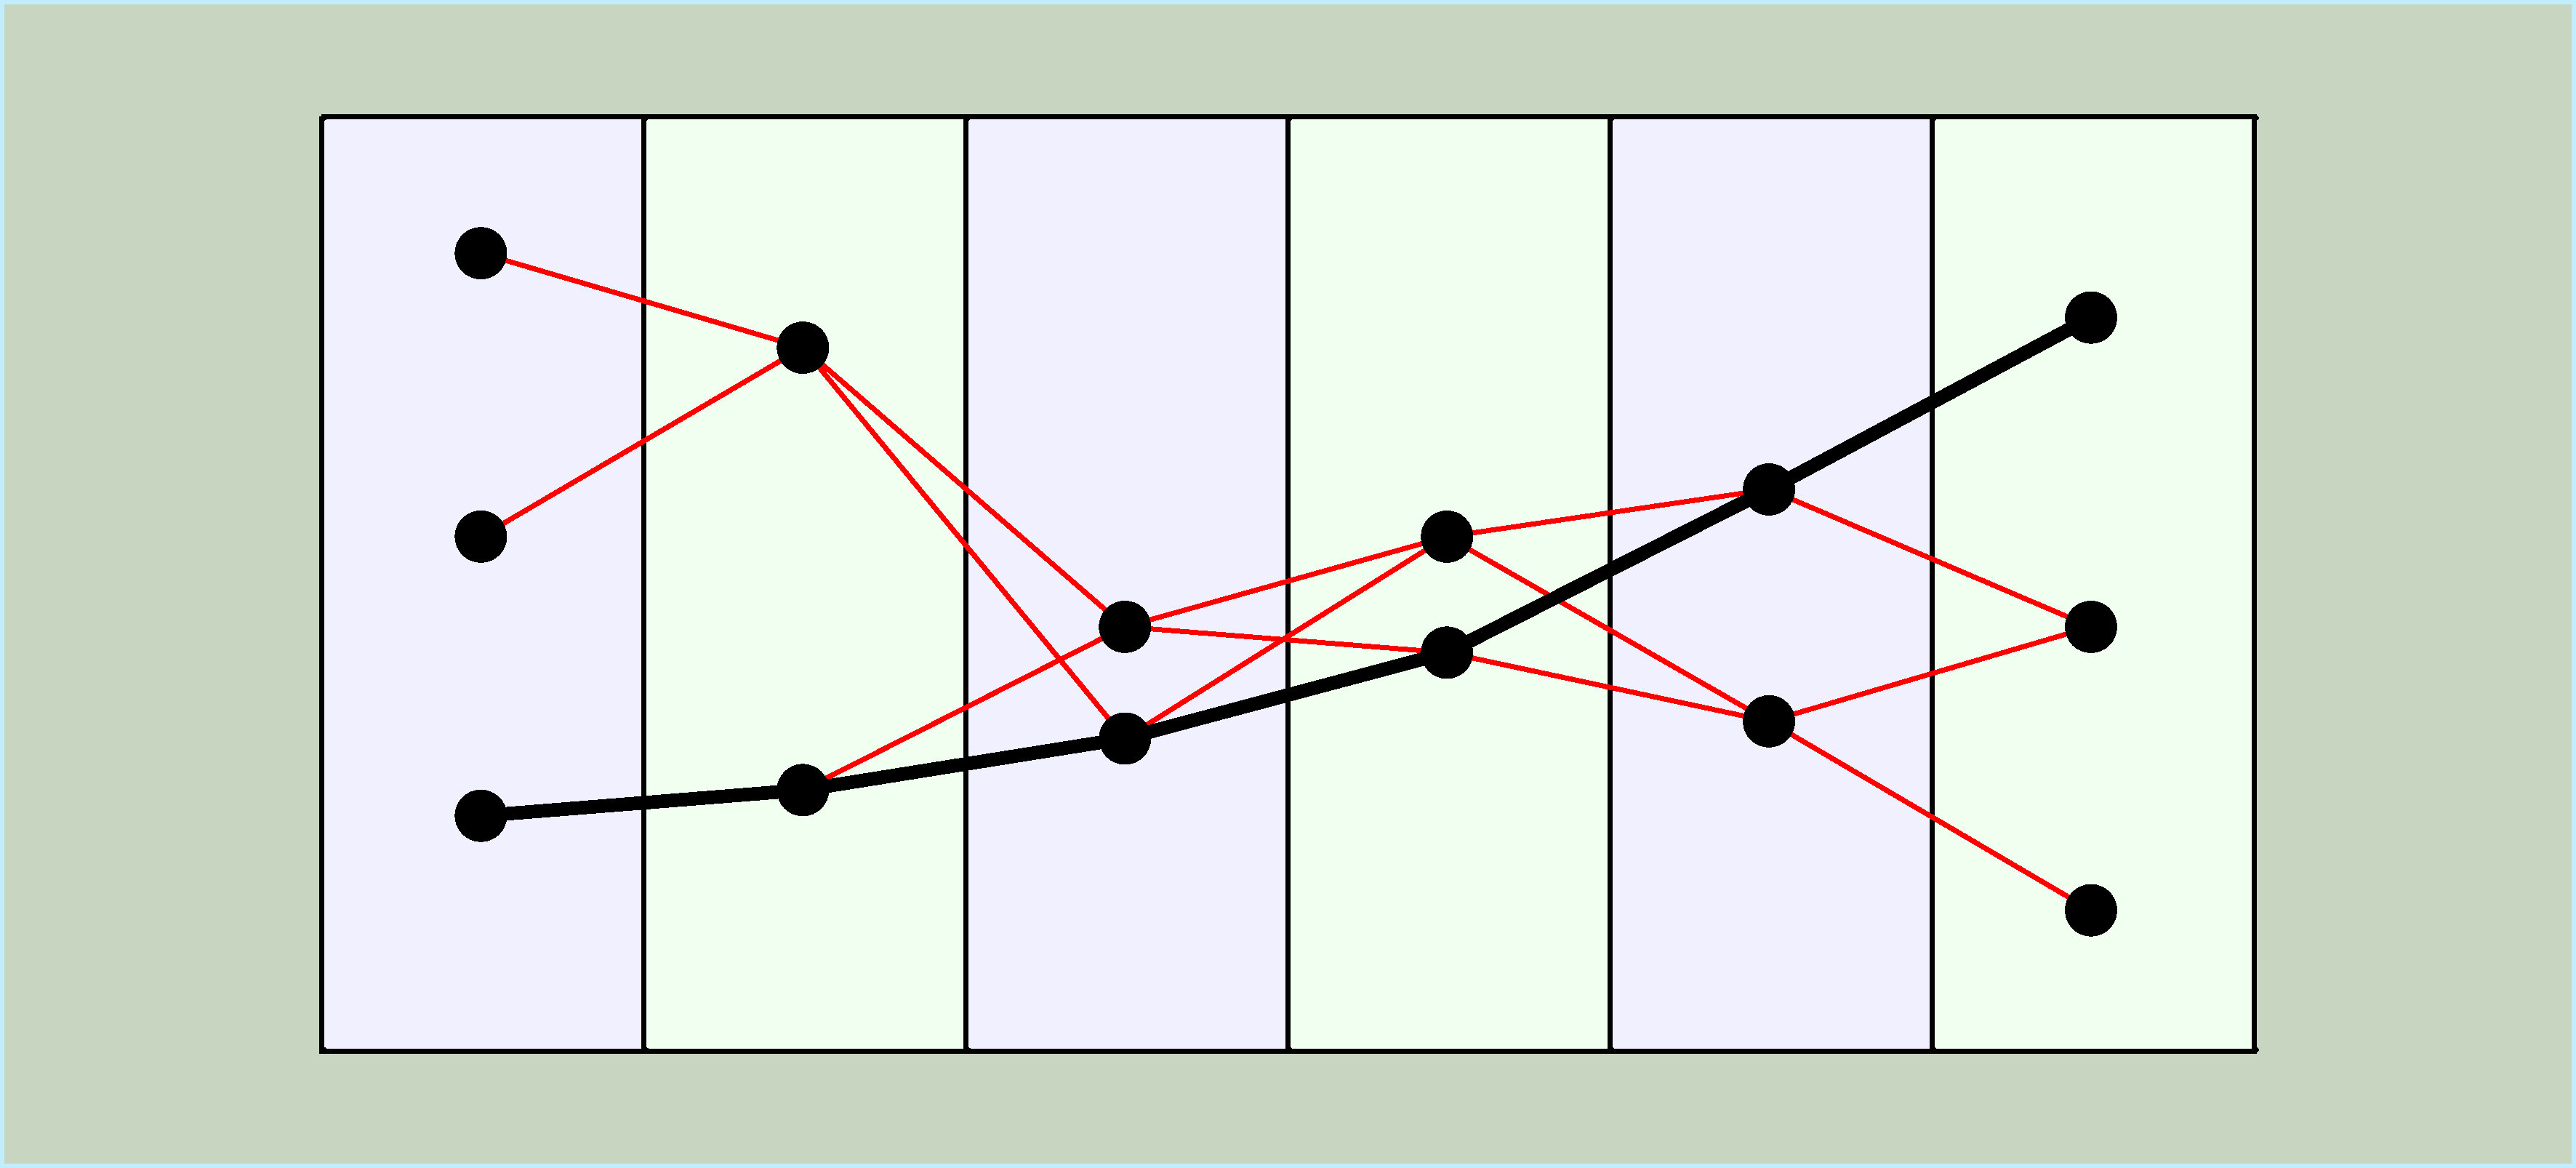
\includegraphics[angle=90,width=1.1in]{images/iden_6_sl.pdf}
  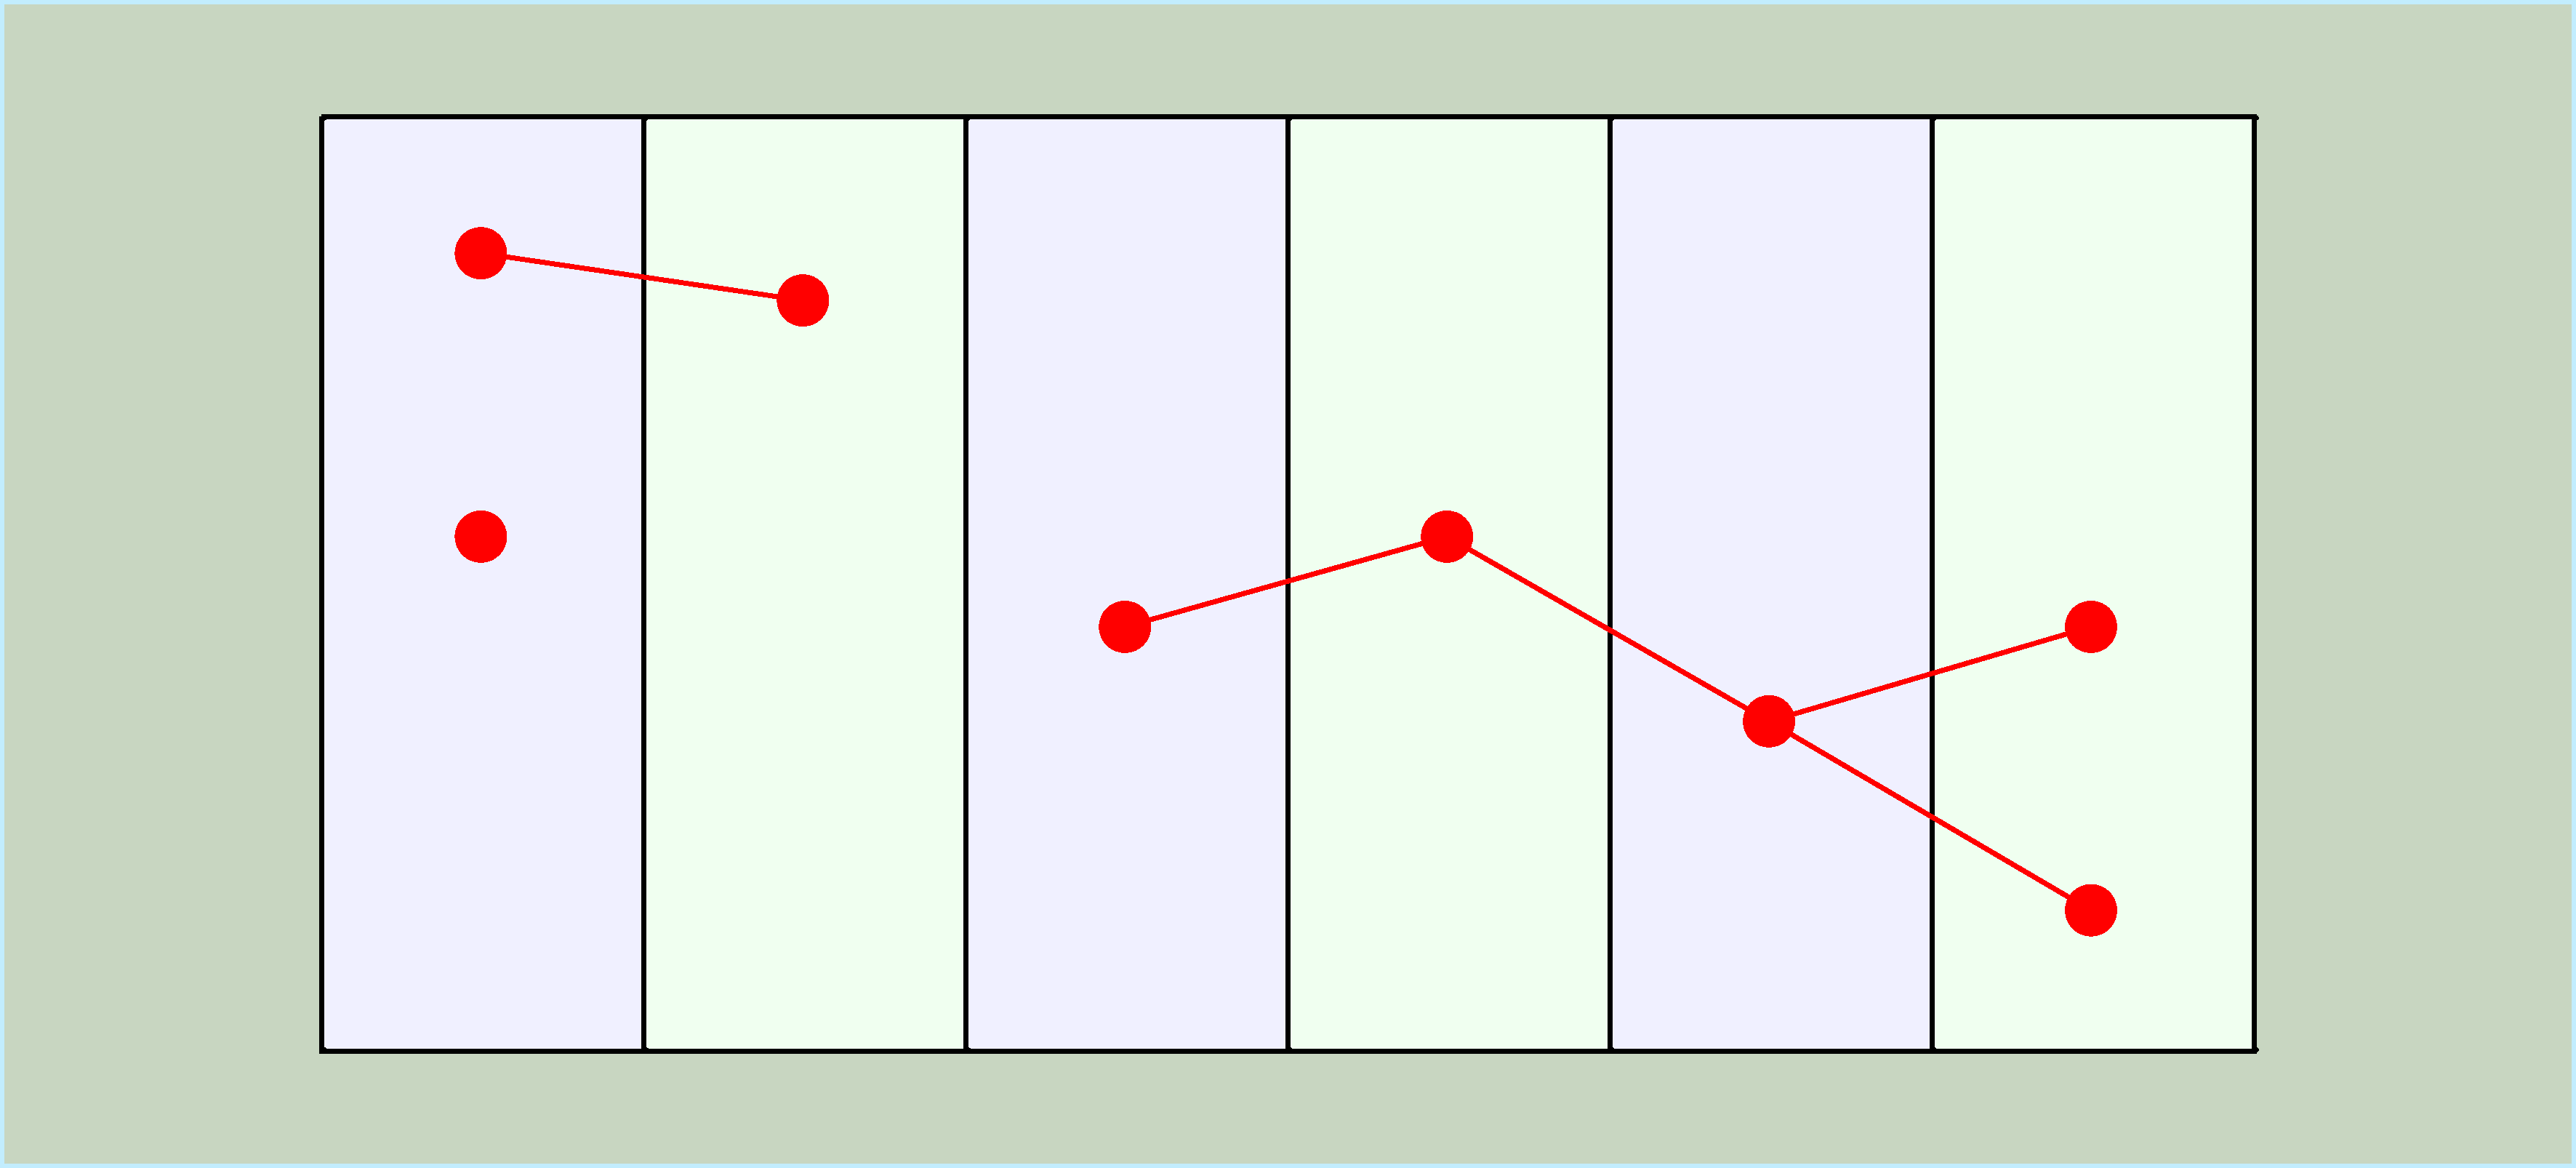
\includegraphics[angle=90,width=1.1in]{images/iden_5_sl_a.pdf}
    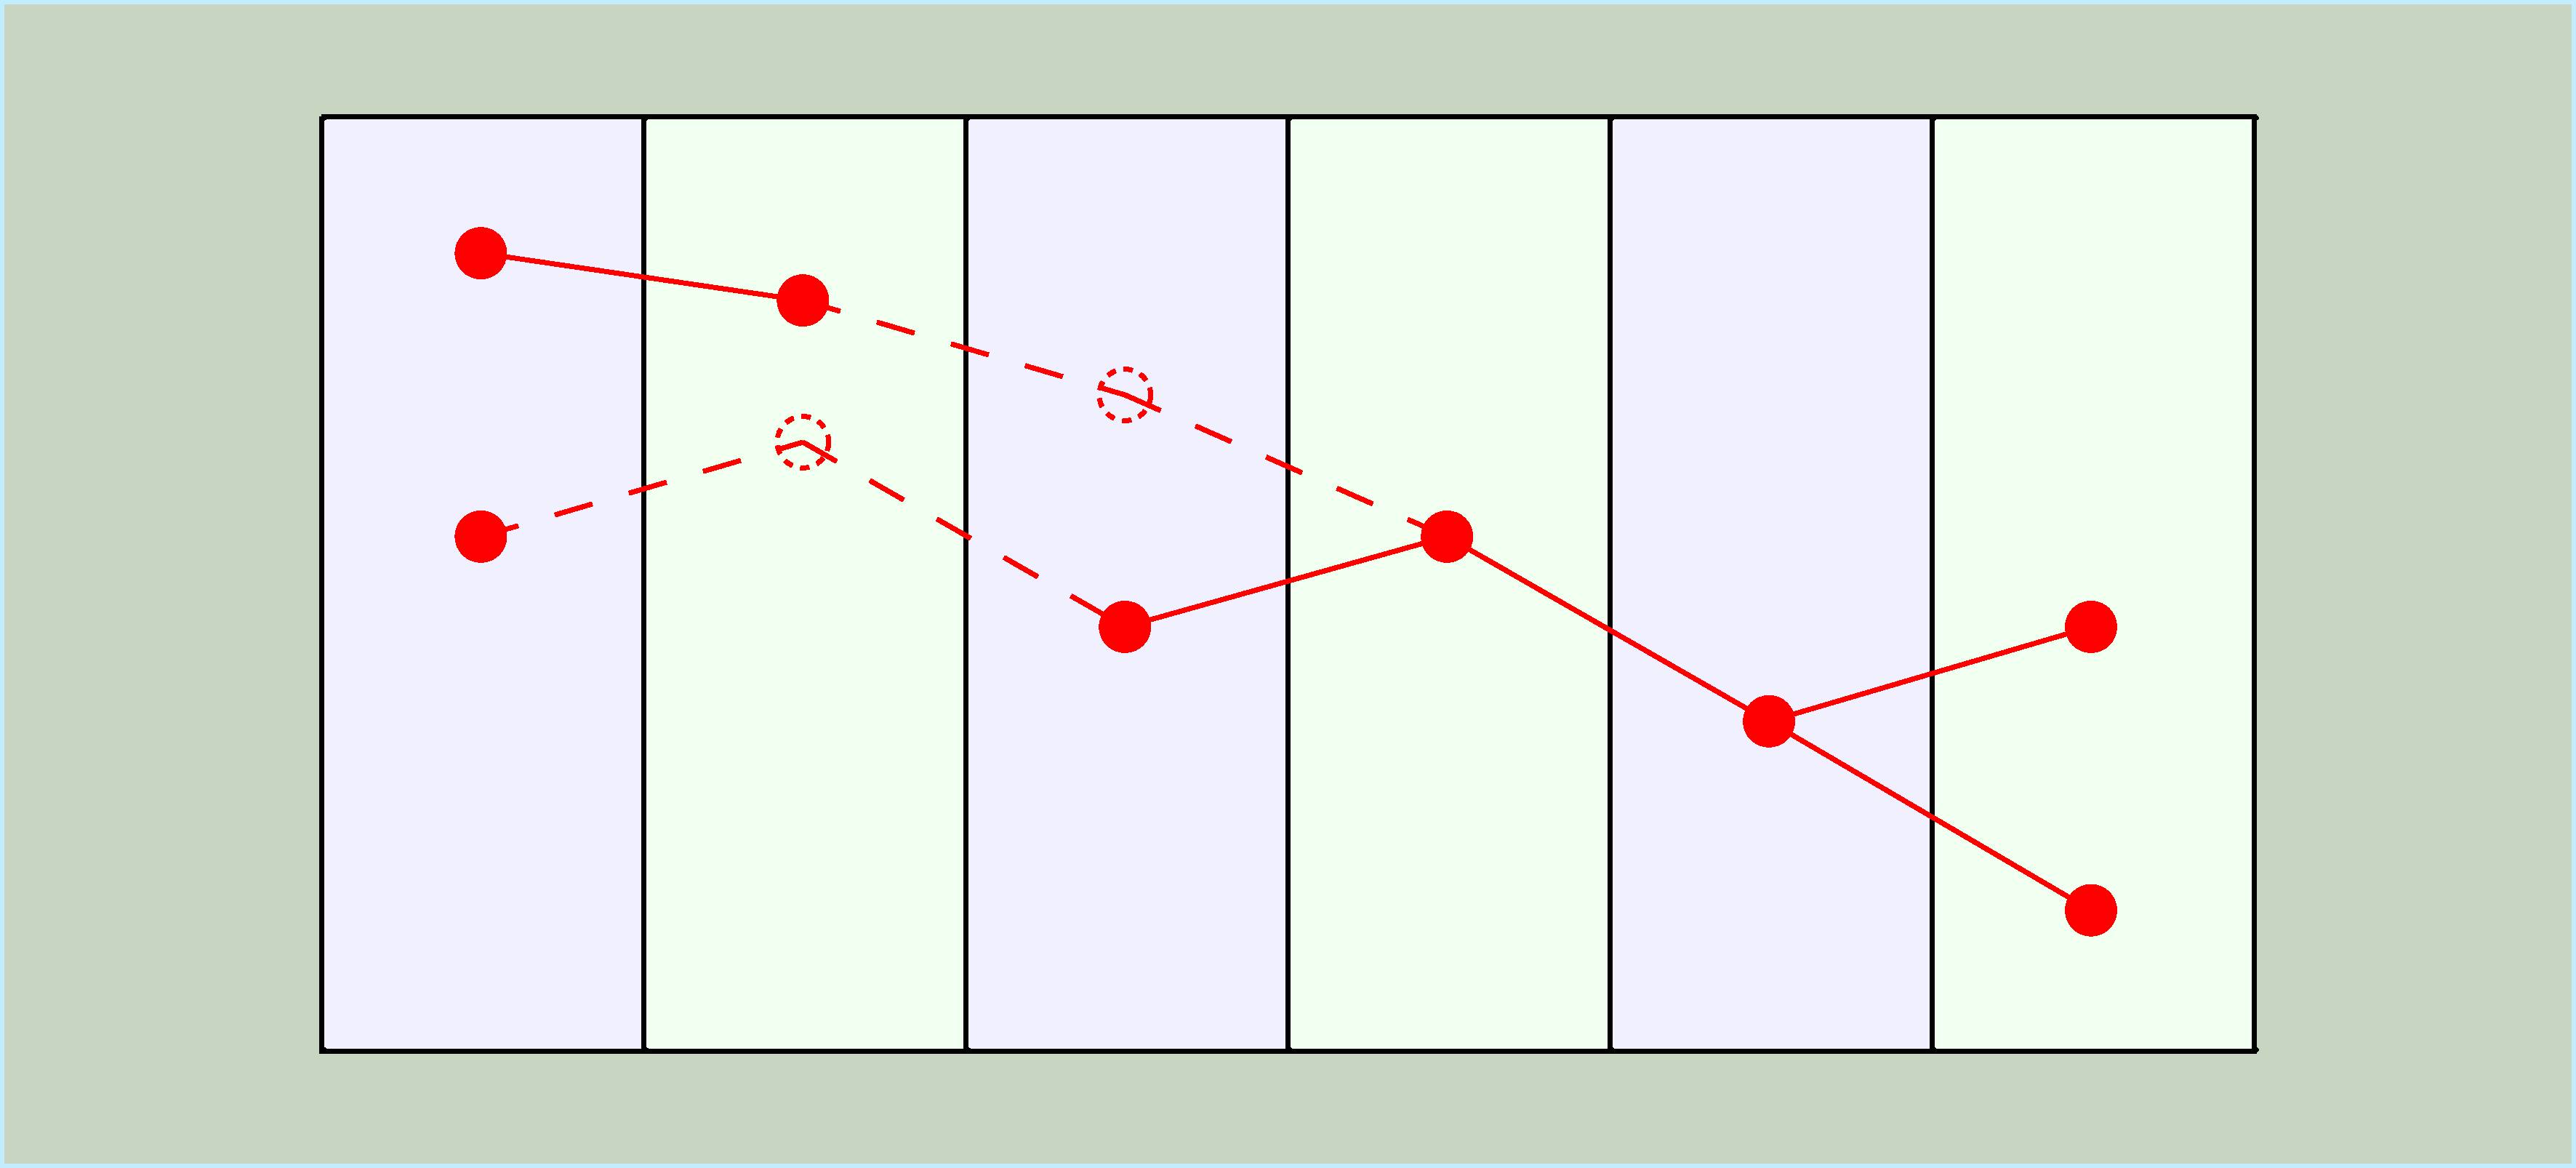
\includegraphics[angle=90,width=1.1in]{images/iden_5_sl_b.pdf}
      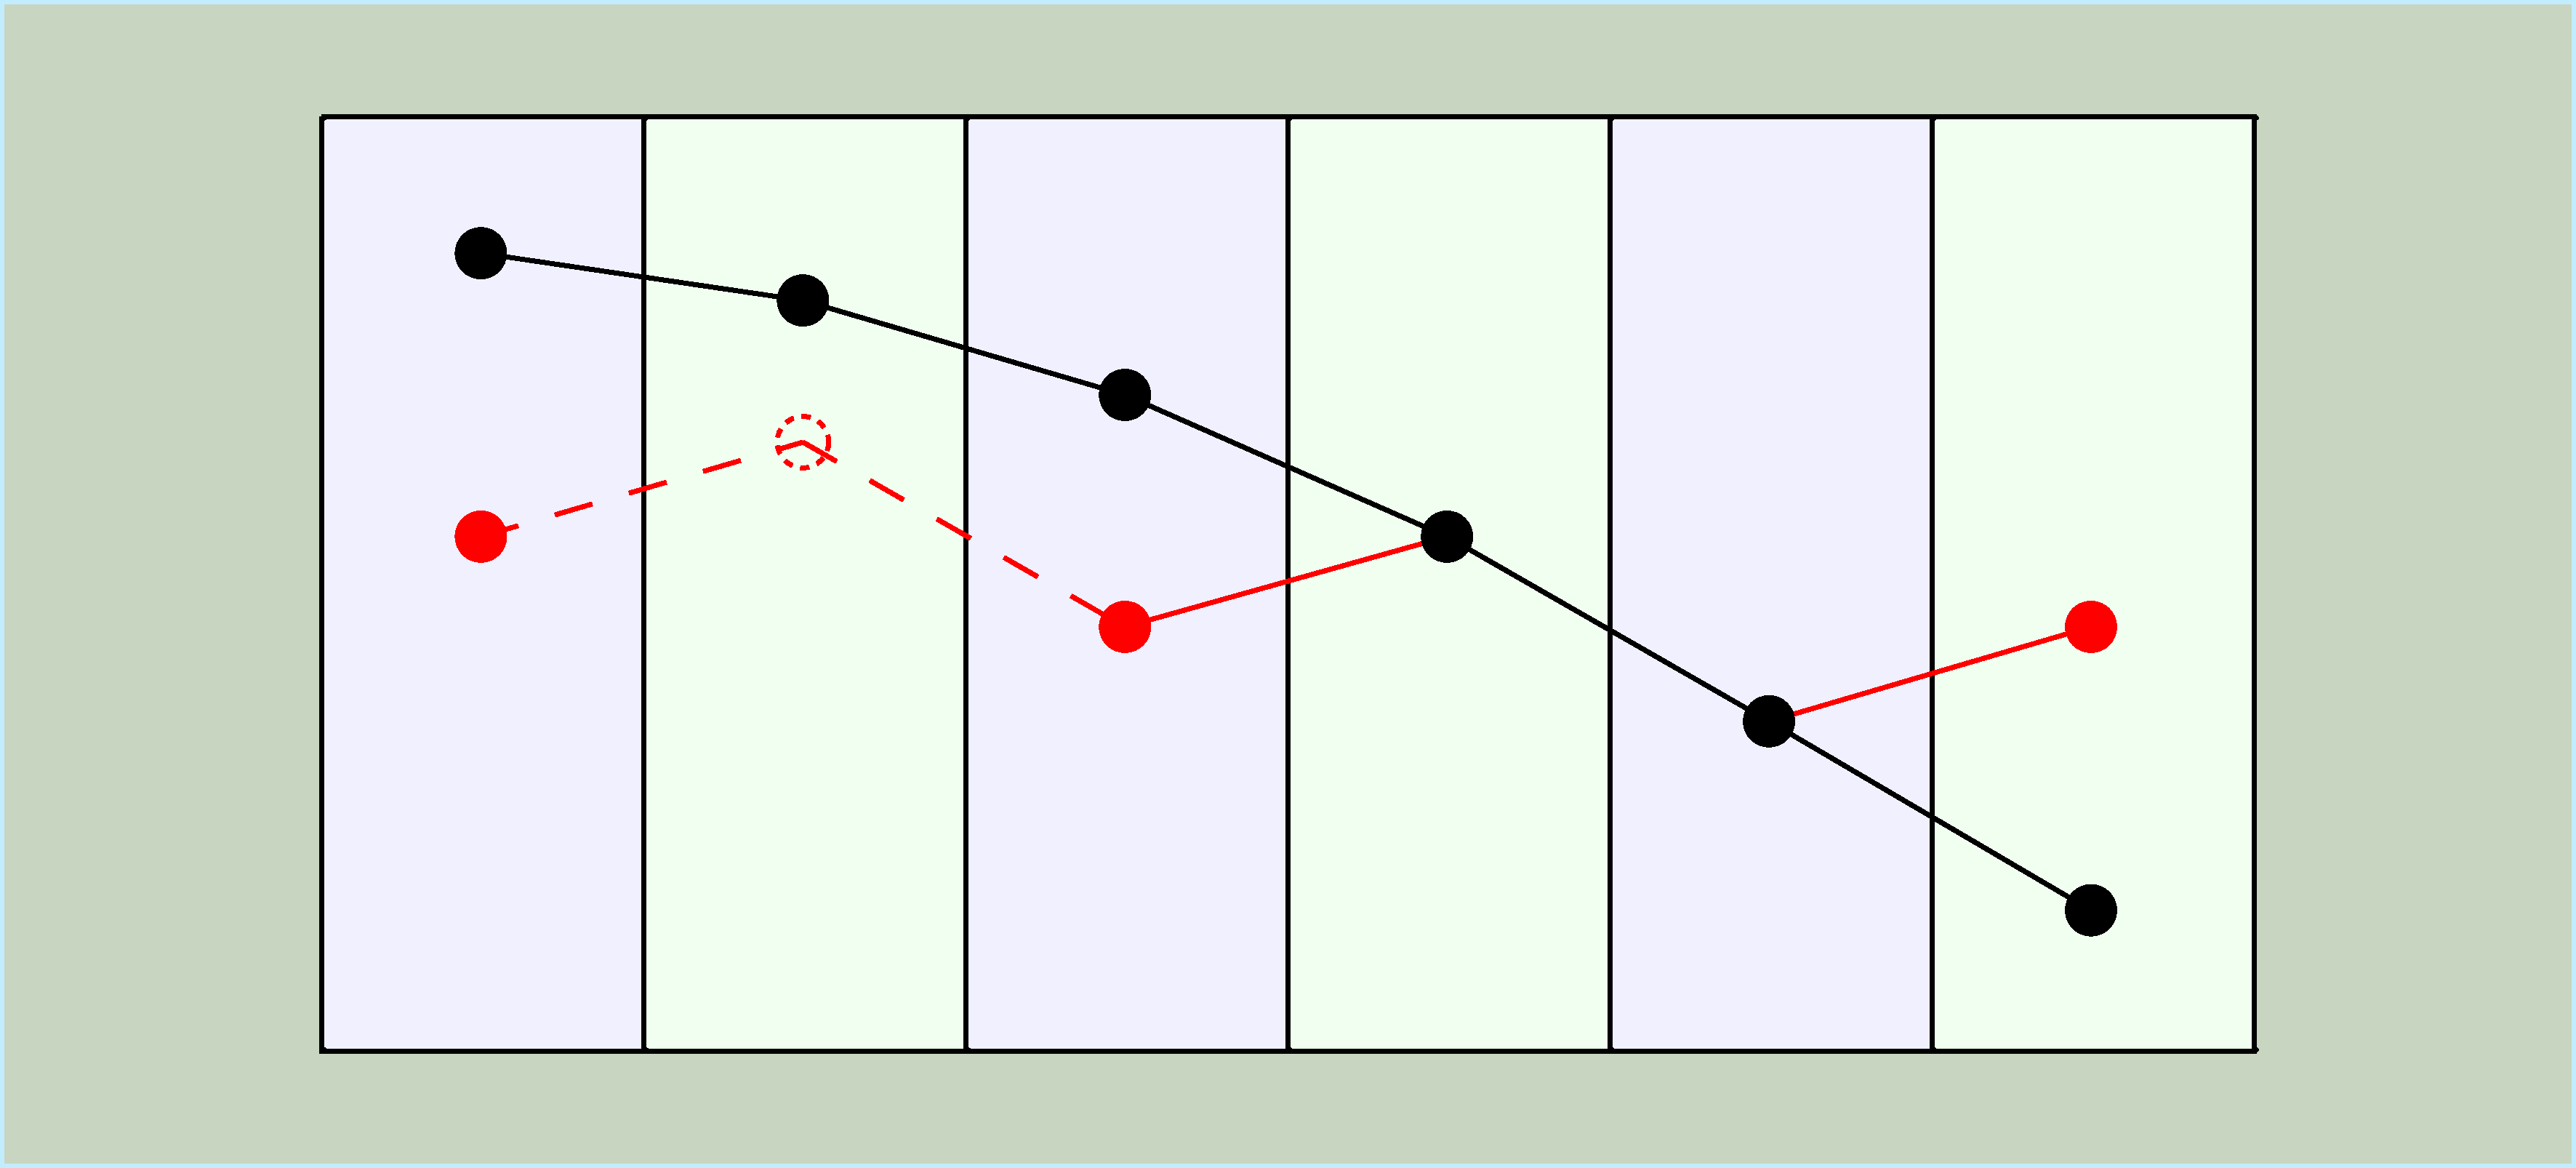
\includegraphics[angle=90,width=1.1in]{images/iden_5_sl_c.pdf}
            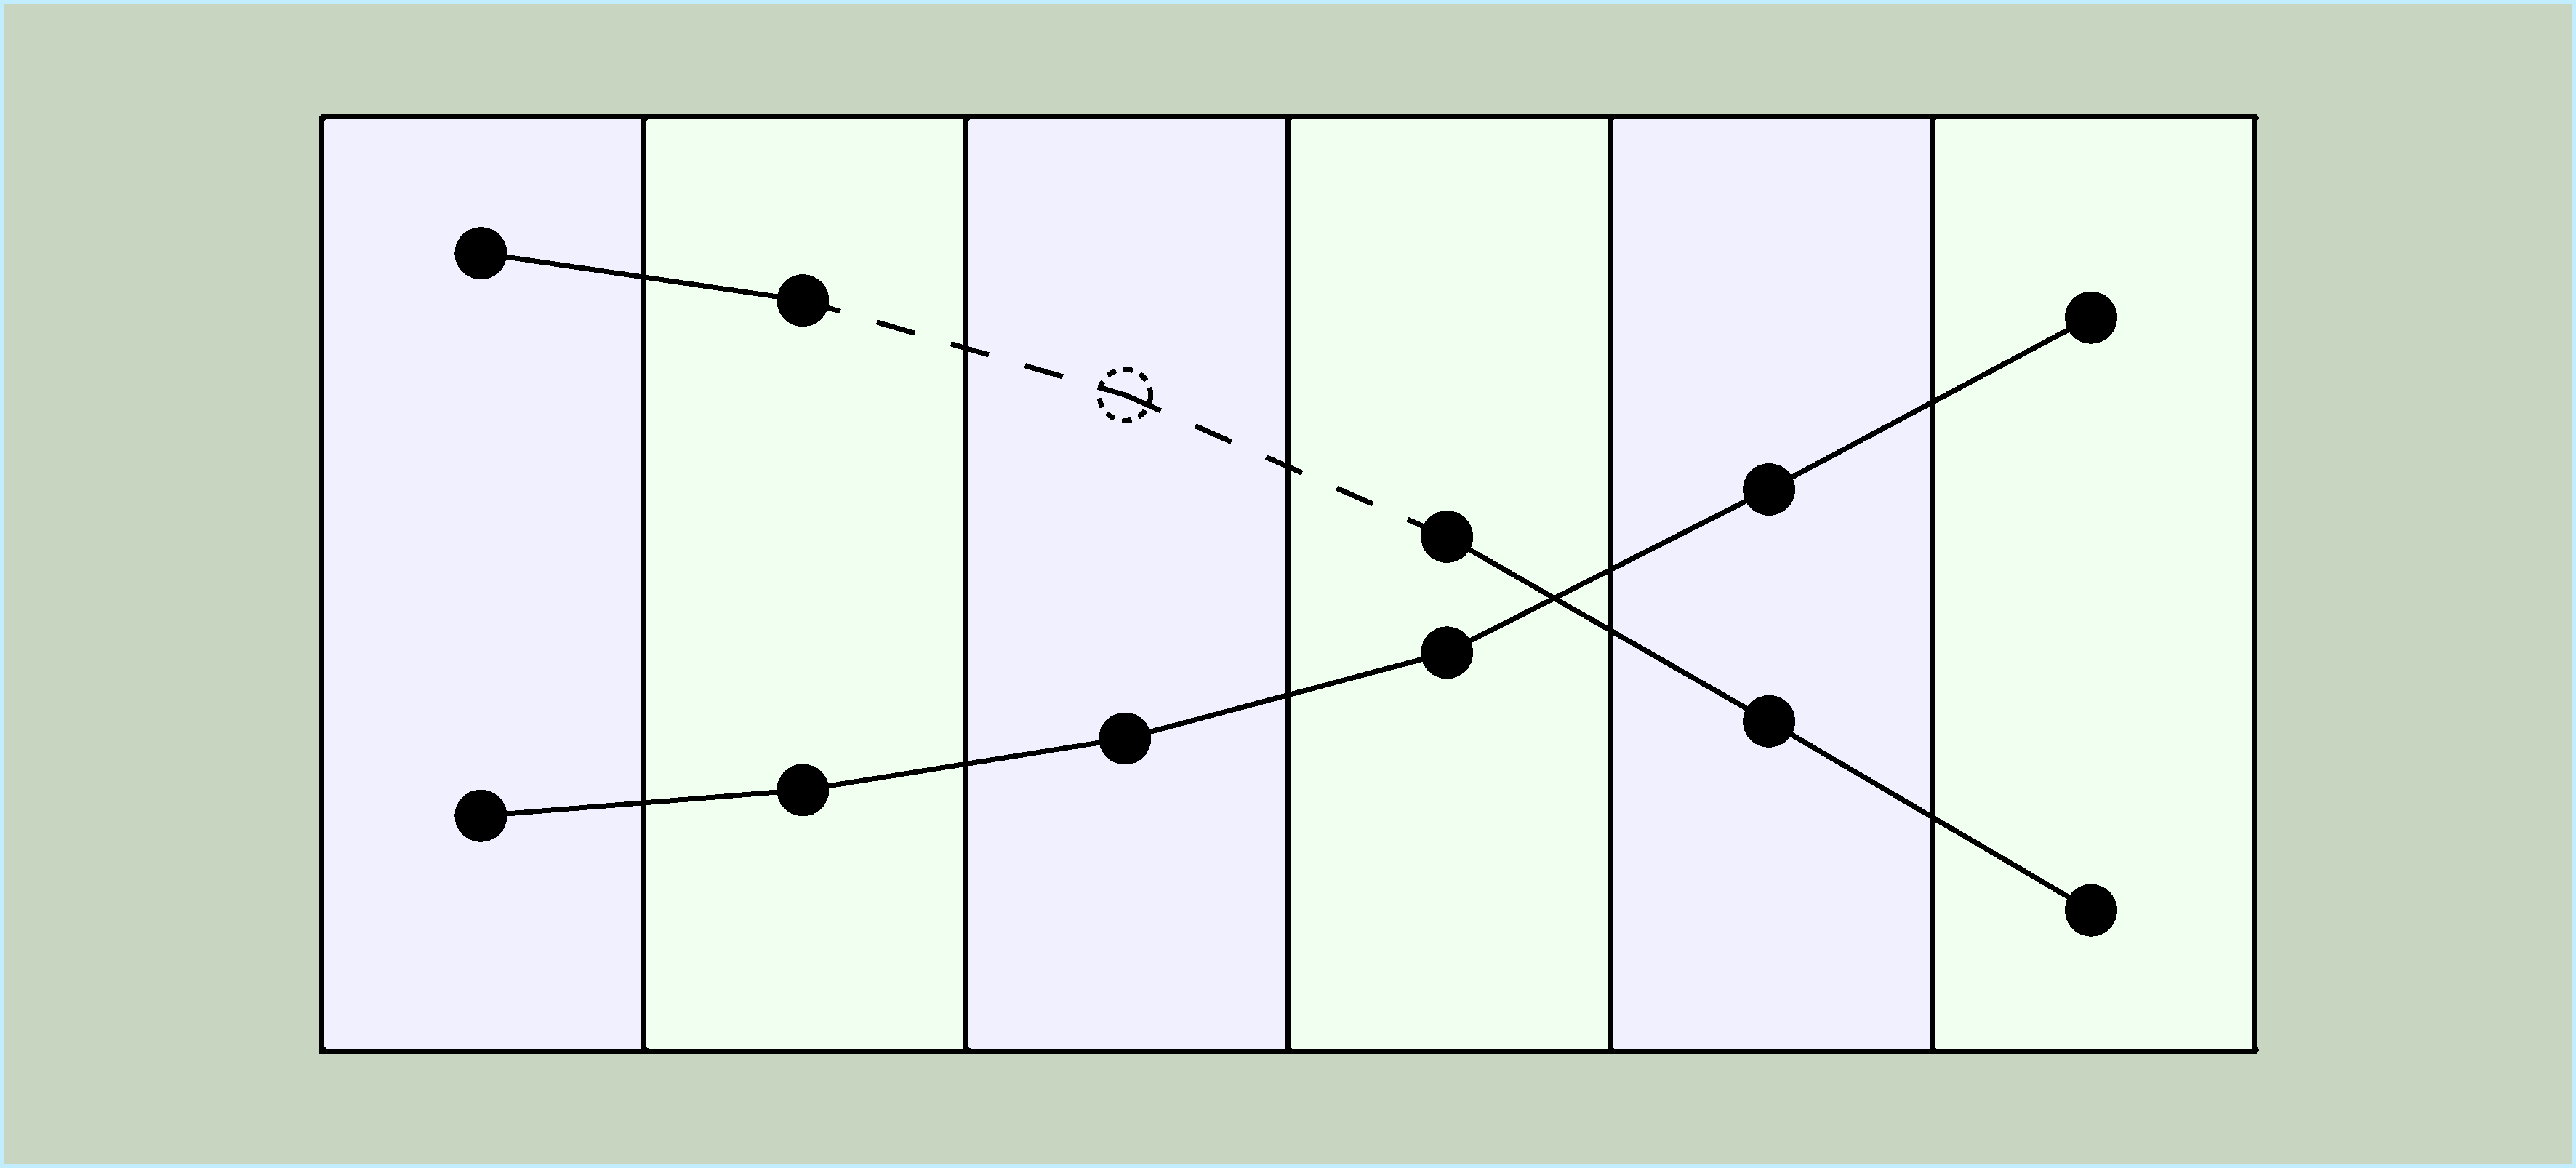
\includegraphics[angle=90,width=1.1in]{images/iden_5_sl_d.pdf}
            
\caption {Stages of Neural Network track identification procedure. 1) identifying 6 super-layer tracks. 2) 
removing all hits belonging to a identified track and constructing 5 super-layer track candidates. 
3) generating pseudo-clusters for 5 super-layer track candidates using corruption fixing auto-encoder. 
4) identify good track candidates from the list of 6 super-layer (one of the super-layers is pseudo-cluster) 
track candidates. 5) isolate both identifies (6 super-layer and 5 super-layer) tracks  for further fitting with 
Kalman-Filter.}
 \label{network:procedure}
 \end{center}
\end{figure}

The second stage of track identification starts by constructing a list of track candidates with combinations 
of 5 clusters out of 6 from all existing clusters (one per super-layer). The candidates that share a cluster with 
tracks identified at the first stage of classification are removed from the list. For each track candidate with a 
missing cluster in one of the super-layers, a pseudo-cluster is generated using the Corruption Auto-Encoder 
Network and the missing super-layer cluster is assigned the inferred value, hence turning all track candidates 
to 6 cluster track candidates. The cured (or fixed) track candidate list is finally passed to the track classifier 
module described above, which evaluates the list isolating candidates with the highest probability of being a 
good track. 

\subsection{Implementation in reconstruction software}

The CLAS12 reconstruction software framework is a Service Oriented Architecture platform (CLARA~\cite{Gyurjyan:2011zz}).
The reconstruction software consists of several microservices, each responsible for processing data from one
detector \cite{Ziegler:2020gsr}. The reconstruction procedure for some of the detector components can also 
be broken down into smaller logical microservices to add some flexibility in changing the implementation of 
the small parts, and provide alternative reconstruction procedures for some of the components. Reconstruction 
of tracks in drift chambers is a complex task and consists of several parts.

The first stage of the process, called clustering service, is to isolate clusters from the hits in drift chambers. 
Once the clusters are isolated, track candidates are formed from all combinations of 6 segments. Once 6 
segment tracks have been identified, the remaining segments are then used to form 5 segments combinations. 
These two steps are known as track-finding or seeding. Both 6 and 5 segments candidates are fitted defining 
the hit positions from the wire coordinates (hit based tracking), resulting in a first list of reconstructed tracks.

In a second stage of the tracking code (time-based tracking), the tracks identified at the previous stage are 
refitted with a Kalman Filter algorithm, which uses drift time information to refine the hit positions. This 
produces the final track list.

\begin{figure}[!ht]
\begin{center}
 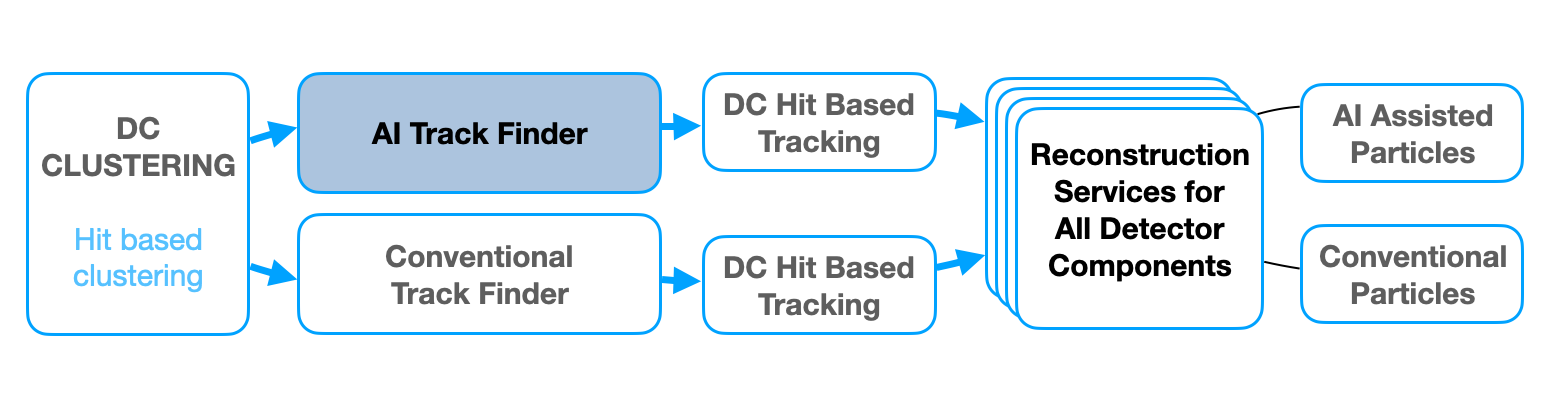
\includegraphics[width=6.0in]{images/CLARA_AI_diagram.png}
\caption {Diagram of the tracking workflow with Artificial Intelligence included. The Workflow is split into 
two parallel branches, one where track-finding is done by the conventional algorithm, and one where only 
AI-isolated tracks are fed to the following stages.}
 \label{recon:diagram}
 \end{center}
\end{figure}

In order to implement our neural network into the reconstruction workflow, we designed two parallel 
branches in the reconstruction code where we run two algorithms to identify good tracks from the 
candidate lists, one based on the conventional algorithm and one based on the neural network. The two 
algorithms store their track suggestions in separate data structures, and pass them to the next stage where 
track parameters are reconstructed by conventional tracking algorithm, first by hit-based fitting and then 
using the Kalman filter. This approach lets us have two parallel outputs from the tracking code that enables 
a detailed comparison of the performance of each method.

\subsection{Software Packages}

As mentioned above, CLAS12 reconstruction is implemented in Java. The final implementation of the the 
track classifier was therefore in Java for easy integration into the reconstruction workflow. The initial tests 
and prototyping were done using the Keras/TensorFlow~\cite{keras-website} (python) package. The final 
implementation was based on the DeepNetts \cite{Sevarac.Z} community edition library (in native Java) 
used for both the track candidate classifier and corruption-recovery auto-encoder. DeepNetts is a light weight
 library with minimal dependencies, which makes it ideal for providing portable code that can be used on variety 
 of platforms without the need of installing large number of platform-dependent packages (like in the case of
  keras/tensorflow). The inference procedure was implemented using Efficient Java Matrix Library (EJML)~\cite{ejml:2021}, 
  which is optimized for speed and is thread safe, matching the requirements of the CLAS12 reconstruction software.

The analysis and data visualization for this article was done using GROOT data visualization package~\cite{groot-github} 
developed for CLAS12 software infrastructure (in Java) and is included in the Java data analysis library for high energy 
physics Jas4pp~\cite{Chekanov:2020bja}.
